%%%%%%%%%%%%%%%%%%%%%%%%%%%%%%%
%   Figures for chapter 3 - 
%%%%%%%%%%%%%%%%%%%%%%%%%%%%%%%

%% \newcommand{\figFrameworkFlow}{
%%     \begin{figure}
%%         \centering
%%         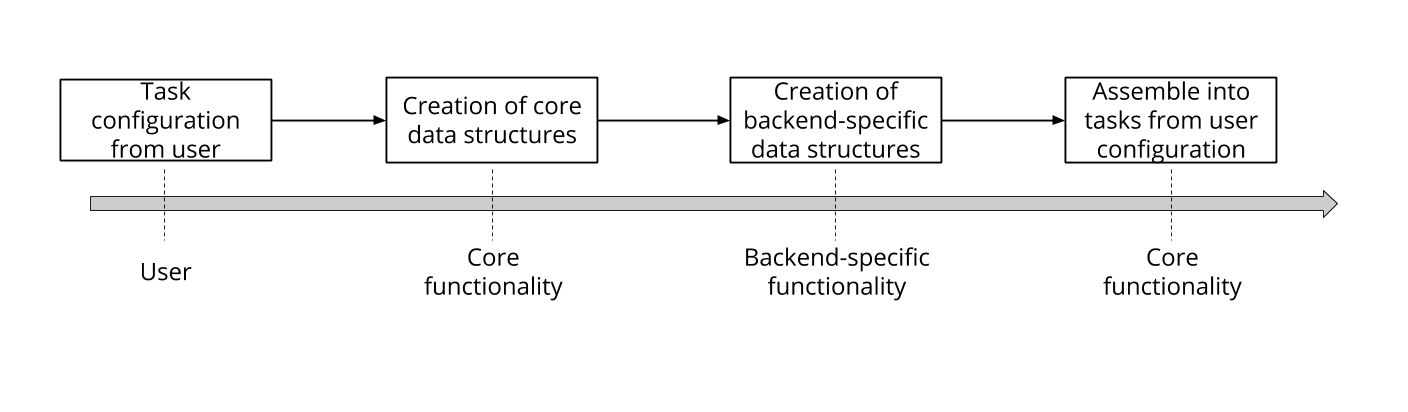
\includegraphics[width=0.9\textwidth]{./chapters/chapter_4/imgs/img_ch4_framework_flow.png}
%%         \caption{Flow of data in the proposed framework}
%%         \label{fig:ch4_proposed_framework_flow}
%%     \end{figure}
%% }

%% \newcommand{\figFrameworkCoreSensor}{
%%     \begin{figure}[!ht]
%%         \centering
%%         \begin{subfigure}[b]{0.3\textwidth}
%%             \centering
%%             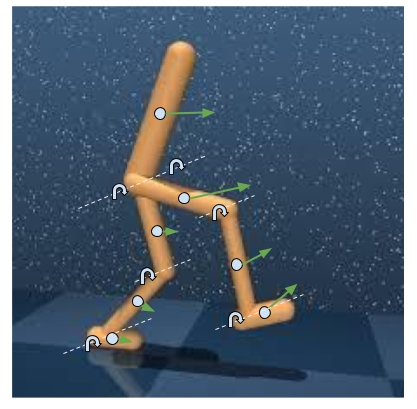
\includegraphics[width=0.9\textwidth]{./chapters/chapter_4/imgs/img_ch4_sensors_core_1.png}
%%             \caption{}
%%             \label{fig:ch4_core_sensor_1}
%%         \end{subfigure}
%%         \begin{subfigure}[b]{0.3\textwidth}
%%             \centering
%%             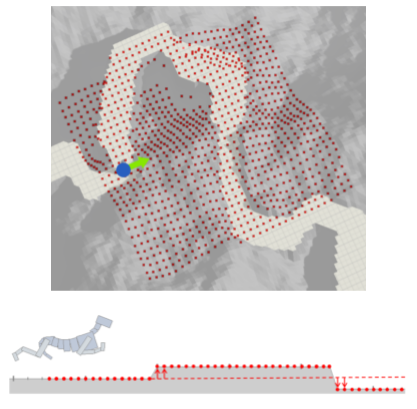
\includegraphics[width=0.9\textwidth]{./chapters/chapter_4/imgs/img_ch4_sensors_core_2.png}
%%             \caption{}
%%             \label{fig:ch4_core_sensor_2}
%%         \end{subfigure}
%%         \begin{subfigure}[b]{0.3\textwidth}
%%             \centering
%%             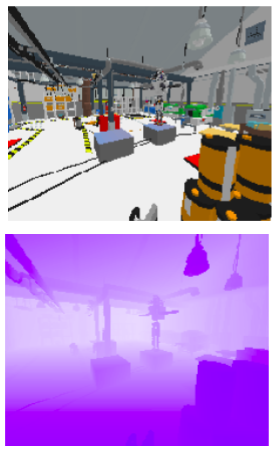
\includegraphics[width=0.9\textwidth]{./chapters/chapter_4/imgs/img_ch4_sensors_core_3.png}
%%             \caption{}
%%             \label{fig:ch4_core_sensor_3}
%%         \end{subfigure}
%%         \caption{Core sensors functionality. a) Intrinsic readings from joints and bodies (adapted from [@CITE]).
%%                                              b) Extrinsic readings from heightmaps of the terrain (adapted from [@CITE,@CITE]).
%%                                              c) Extrinsic readings from rgb and depth images of the agent view (adapted from [@CITE]).}
%%         \label{fig:ch4_core_sensor_functionality}
%%     \end{figure}
%% }

\newcommand{\figBenchmarkControlSuite}{
	\begin{figure}
		\centering
		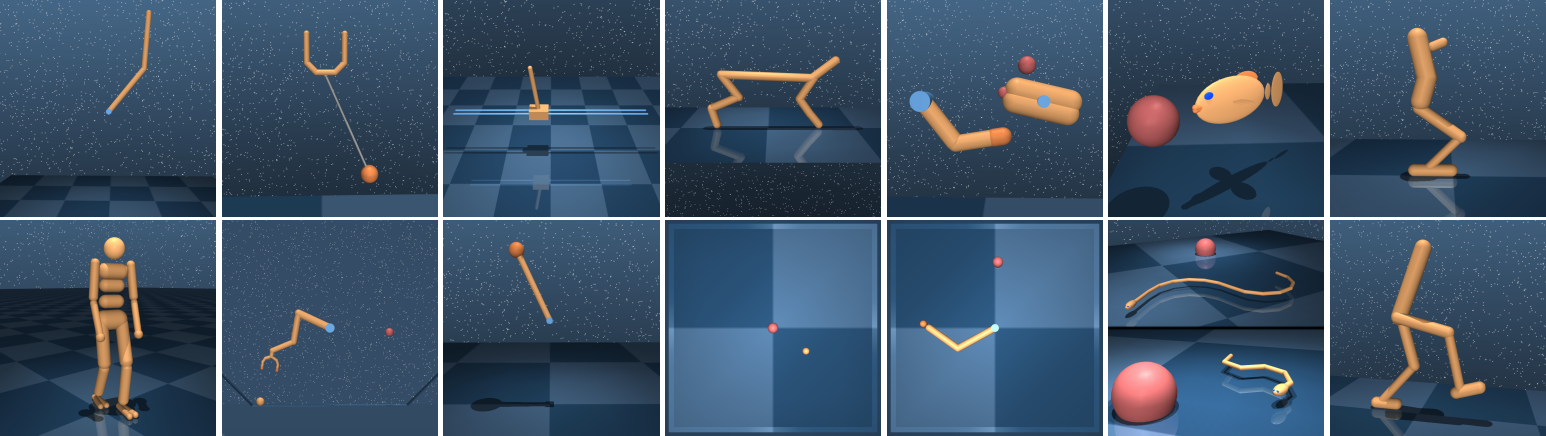
\includegraphics[width=0.9\textwidth]{./chapters/chapter_3/imgs/img_ch3_controlsuite.png}
		\caption{Models available in the Controlsuite benchmark. 
				 Extracted from \citet{Controlsuite}}
	    \label{fig:ch3_controlsuite}
	\end{figure}
}

\newcommand{\figBenchmarkOpenAIGymMujoco}{
    \begin{figure}[!ht]
        \centering
        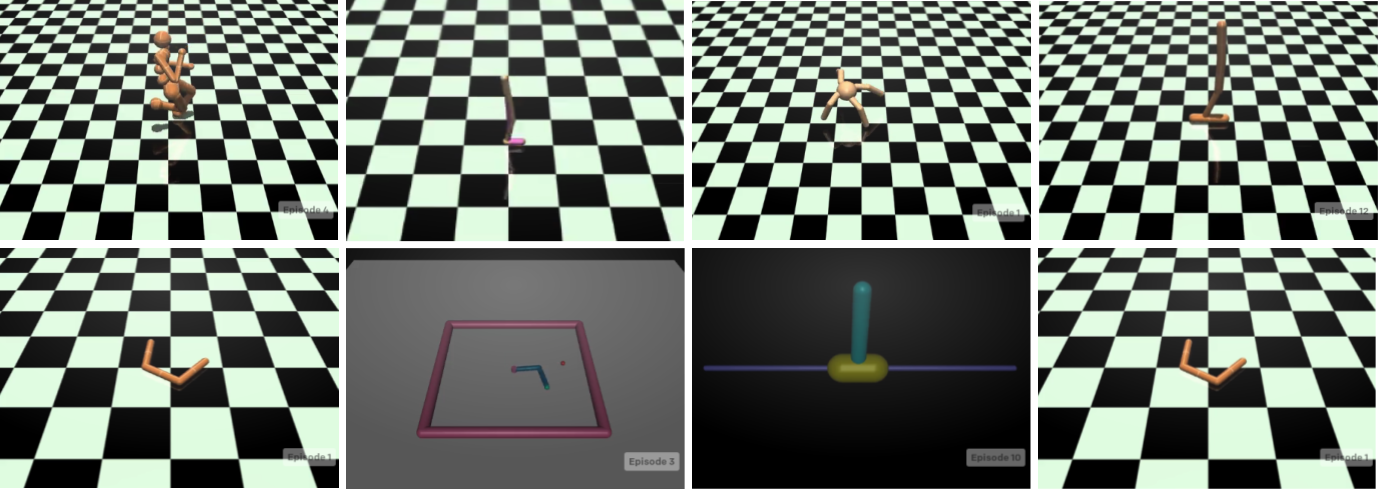
\includegraphics[width=0.9\textwidth]{./chapters/chapter_3/imgs/img_ch3_openaigym_mujoco.png}
        \caption{Models available in the OpenAI-gym benchmark with mujoco as backend. 
                 Extracted from \citet{Gym}}
        \label{fig:ch3_openaigym_mujoco}
    \end{figure}
}

\newcommand{\figBenchmarkOpenAIGymRoboschool}{
    \begin{figure}[!ht]
        \centering
        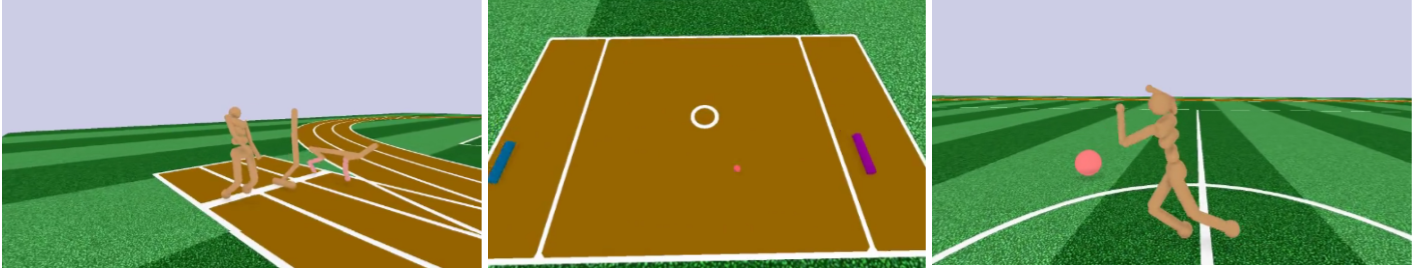
\includegraphics[width=1.0\textwidth]{./chapters/chapter_3/imgs/img_ch3_openaigym_roboschool.png}
        \caption{Models available in the OpenAI-gym benchmark with Bullet as backend. 
                 Extracted from \citet{Roboschool}}
        \label{fig:ch3_openaigym_roboschool}
    \end{figure}
}

\newcommand{\figBenchmarkRllabClassic}{
    \begin{figure}[!ht]
        \centering
        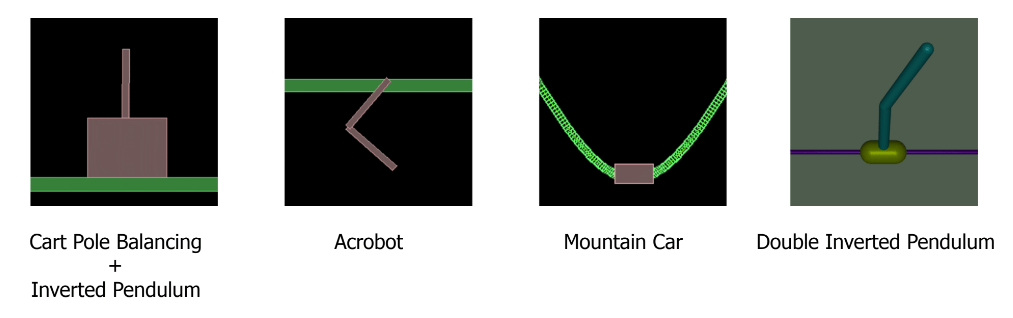
\includegraphics[width=1.0\textwidth]{./chapters/chapter_3/imgs/img_ch3_rllab_classic.png}
        \caption{Models available in the Rllab classic benchmark. Extracted from \cite{Rllab}}
        \label{fig:ch3_rllab_classic}
    \end{figure}
}

\newcommand{\figBenchmarkRllabLocomotion}{
    \begin{figure}[!ht]
        \centering
        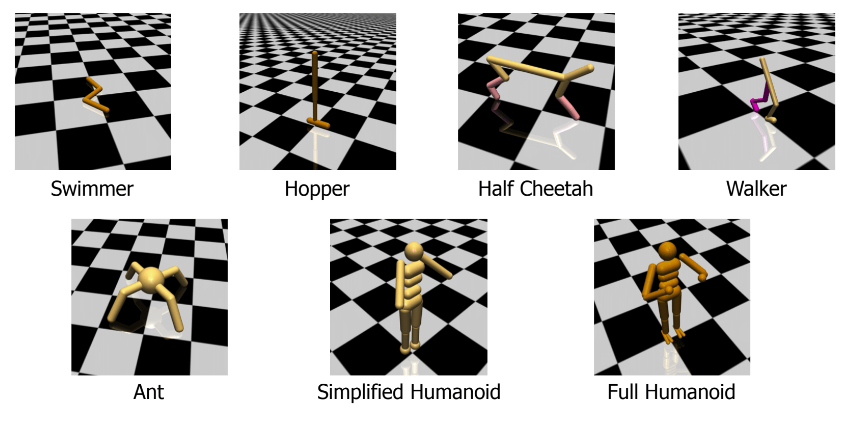
\includegraphics[width=0.9\textwidth]{./chapters/chapter_3/imgs/img_ch3_rllab_locomotion.png}
        \caption{Models available in the Rllab locomotion benchmark. Extracted from \citet{Rllab}}
        \label{fig:ch3_rllab_locomotion}
    \end{figure}
}

\newcommand{\figBenchmarkRllabHierarchical}{
    \begin{figure}[!ht]
        \centering
        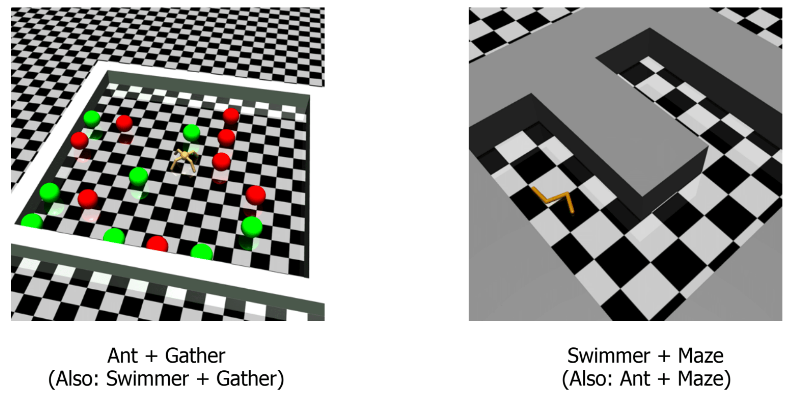
\includegraphics[width=0.9\textwidth]{./chapters/chapter_3/imgs/img_ch3_rllab_hierarchical.png}
        \caption{Models available in the Rllab hierarchical benchmark. Extracted from \citet{Rllab}}
        \label{fig:ch3_rllab_hierarchical}
    \end{figure}
}